\documentclass[tikz,border=4pt]{standalone}
\usetikzlibrary{shapes.geometric}

\definecolor{cA}{HTML}{0B1F4D}
\definecolor{cB}{HTML}{1B4F9C}
\definecolor{cC}{HTML}{2C7FB8}
\definecolor{cD}{HTML}{6BA3E0}
\definecolor{cE}{HTML}{9DC0EF}
\definecolor{cF}{HTML}{C8DBF8}
\definecolor{lblcol}{HTML}{2E6FD0}

\begin{document}
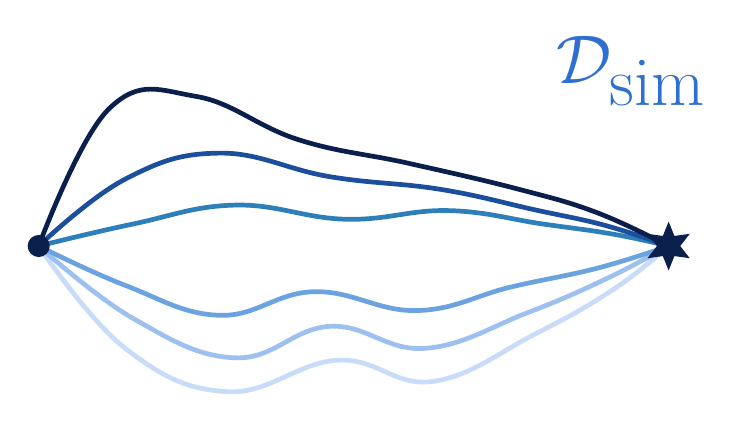
\begin{tikzpicture}[x=1cm,y=1cm,line cap=round,line join=round]

  \begin{scope}[line width=1.7pt]
    \draw[cF] plot[smooth,tension=0.7] coordinates
      {(0,0) (1.1,-1.30) (2.4,-1.85) (3.8,-1.45) (5.0,-1.72) (6.3,-1.12) (7.3,-0.55) (8,0)};
    \draw[cE] plot[smooth,tension=0.7] coordinates
      {(0,0) (1.2,-0.92) (2.5,-1.42) (3.7,-1.02) (4.9,-1.30) (6.2,-0.85) (7.2,-0.42) (8,0)};
    \draw[cD] plot[smooth,tension=0.7] coordinates
      {(0,0) (1.1,-0.50) (2.3,-0.88) (3.5,-0.58) (4.8,-0.82) (6.0,-0.52) (7.1,-0.28) (8,0)};
    \draw[cC] plot[smooth,tension=0.7] coordinates
      {(0,0) (1.2,0.28) (2.5,0.52) (3.9,0.34) (5.2,0.45) (6.4,0.28) (7.3,0.15) (8,0)};
    \draw[cB] plot[smooth,tension=0.7] coordinates
      {(0,0) (1.1,0.85) (2.3,1.18) (3.7,0.88) (5.1,0.72) (6.3,0.46) (7.2,0.26) (8,0)};
    \draw[cA] plot[smooth,tension=0.7] coordinates
      {(0,0) (0.9,1.75) (2.0,1.90) (3.3,1.35) (4.7,1.05) (6.1,0.72) (7.1,0.42) (8,0)};
  \end{scope}

  \fill[cA] (0,0) circle (0.14);
  \node[star,star points=6,star point ratio=2.1,fill=cA,draw=none,
        minimum size=0.62cm,inner sep=0pt] at (8,0) {};

  \node[anchor=north east,lblcol] at (8.6,2.78)
    {\fontsize{34}{34}\selectfont $\mathcal{D}_{\mathrm{sim}}$};

\end{tikzpicture}
\end{document}
